\documentclass[
	12pt, 
]{fphw_assignment_toc}

\usepackage{my_packages}
\usepackage{graphicx}
%\geometry{
% a4paper,
%% total={170mm,257mm},
% left=20mm,
%% top=20mm,
% }
%------------------------------------------------------------------------------------

\title{Lab Assignment 6}        % Assignment title
\author{Devansh Tanna}    % Student name
\roll{2019A3PS0158P}                    % Class roll
% \class{My Class}              % Class
% \session{My Session}             % Session
\email{f20190158@pilani.bits-pilani.ac.in}
\date{\today}     % Due date
\institute{Department of Electrical and Electronics}              % Institute or school name
\course{Communication System}                            % Course or course name


%------------------------------------------------------------------------------------
\addbibresource{ref.bib} 

\setcounter{secnumdepth}{-2} 
%\renewcommand{\thesection}{}  % https://tex.stackexchange.com/a/30202/114006
%------------------------------------------------------------------------------------
\begin{document}
\maketitle
\newpage
\pagenumbering{gobble}    % to remove the page numbering
\pdfbookmark[section]{\contentsname}{toc}
\tableofcontents
\newpage
\pagenumbering{arabic}          % to start the page numbering

%-----------------------------------------

\section{Python Task 1}
\begin{problem}
 | Generate three message signals as $m_1(t) = \cos(2\pi Nt)$, $m_2(t) = 2N\text{sinc}(2N\pi t)$, and raised cosine pulse$m_3(t) = 200\frac{\cos(\pi 200 t)}{1-4000t^2}\text{sinc}(\pi 200 t)$ each with duration one second. Randomly select one of the message signals and use DSB-SC to modulate the carrier of frequency 1 KHz and amplitude 2 Volts. Transmit the DSB-SC signal over a band-limited channel of appropriate bandwidth. Add AWGN $n(t) \sim (0, 0.01)$. Demodulate the signal using synchronous detector. Synchronous detector is implemented by multiplying the received signal with carrier signal followed by a low pass filter. Plot the modulated and demodulated signal both in time and frequency domain using the real time code for 30 seconds. Take $N$ as the sum of the last three digits of your BITS ID.
\end{problem}

\subsection{Code}

\noindent
\lstset{style=pystyle}
\lstinputlisting[language=Python]{../Task1.py}

\subsection{Results}
%\newline
\noindent

Here we have transmitted sine pulse which is modulated by carrier of frequency $f_c$. So for demodulation we will multiply again by carrier signal which shifts signal at $f=0$ and there will be 2 components at $f=2f_c$ which can remove by Low Pass Filter of bandwidth $f_c$ or $B$(Bandwidth of $m(t)$). \\

By running code repeatedly we can check for different pulses.

\begin{figure}[ht!]
 \centering
 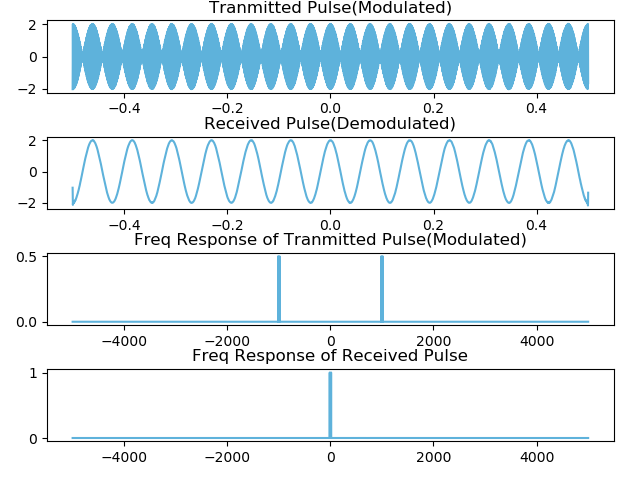
\includegraphics[scale=0.7]{../Task1.png}
\end{figure}
%\subsection{Results}
%\end{mdframed}
% \rule{7in}{2.8pt}
% \begin{figure}[!ht]
%   \centering

%   \caption{ \lipsum[5][2]\cite{book:griffiths}}
%   \label{fig:fig1}
% \end{figure}

% \newpage
\newpage
\section{Python Task 2}
\begin{problem}
Repeat the task 1 if the demodulation is done using envelope detector. The envelope detector is implemented using the MATLAB function hilbert. Say, the received modulated signal is $x_t$, then use $y_t = \text{hilbert}(x_t)\cdot e^{-j 2\pi f_c t}$. The exponential signal is multiplied to shift the modulated signal from bandpass to low pass.
\end{problem}
\subsection{Code}

\noindent
\lstinputlisting[language=Python]{../Task2.py}
% \begin{figure}[!ht]
%   \centering

%   \caption{ \lipsum[5][2]\cite{book:griffiths}}
%   \label{fig:fig1}
% \end{figure}
\subsection{Results}
%\newline
\noindent
\begin{figure}[ht!]
 \centering
 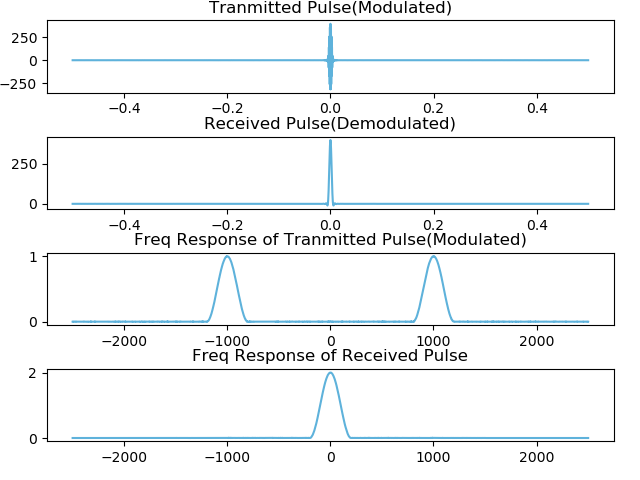
\includegraphics[scale=0.7]{../Task2.png}
\end{figure}
\newpage
As we can see, first Raised Cosine Pulse has been tranmitted with carrier frequency 1 kHz. For receiving, we used hilbert transform function. which gives analytical signal as output, i.e. $H(x_t) = m(t)\cdot e^{j 2\pi f_c t}$ after which we can use frequency translation to obtain the message signal $m(t)$. So , we used envelope detection for removing higher frequency component using Hilbert Transform. \\

By running code, different times we can obtain different transmitting pulses.
%\phantomsection   % 
\printbibliography[heading=bibintoc, title={References}]

\end{document}